\section{Tutorial}
\label{sec:tutorial}
\writer{María}

This section is a practical guide that will show you the basic functionality of the ePNS Petri net simulation system;
the tutorial will go through a simple example to allow you to learn how to use it.

Imagine that you want to simulate a scenario in which a red cube follows a circular line when you press a button. 
First, you need to model the corresponding Petri net where places are visually represented by an image in a 
2D plane \index{2D plane} (in this case, the line and the button), and tokens can represent 3D objects 
\index{3D object} moving on top of the 2D image (in this case, the cube following the line). Transitions have no 
visual representation, but they are of course still necessary for the proper performance of the Petri net. 
The model designed for this scenario could be the one shown in Figure \ref{fig:basic_pn}.

\begin{figure}[htp]
    \begin{center}
    \begin{petri}
        \node at (0, 0) [place] (track) {};
        \node at (3, 2) [inputplace] (semaphore) {};
        \node at (3, 0) [transition] (connection) {};
        \node at (0, 0) [token] {};
        \draw [->,arc] (track) to [out=30,in=150] (connection);
        \draw [->,arc] (connection) to [out=210,in=330] (track);
        \draw [->,arc] (semaphore) -- (connection);
        \draw [-,arc] (2.8, 2.2) -- (3.2, 1.8);
        \draw [-,arc] (2.8, 1.8) -- (3.2, 2.2);
    \end{petri}
    \caption{Petri net model}
    \label{fig:basic_pn}
    \end{center}
\end{figure}

The place on the left is the one that will represent the circular line, and the one with the dashed line 
will represent the button. Note that this second place is not an ordinary place: it is an \textit{input place} 
\index{input place}, where tokens can be externally inserted during the simulation. When the button is clicked, a 
token will appear in that input place, and the transition will be fired. In an ordinary Petri net, when this happens
the tokens in the transition's source places are removed from said places and new ones appear in the transition's target 
places. However, \epns{} offers the posibility of putting identities to arcs to prevent tokens from being destroyed in the 
process and preserve its appearance (if it's a cube, a train, a car...) during the simulation. \index{ePNS Petri net!attributes!identity}

The model can be created using the Petri net editor \index{editors!Petri net} with \epns's custom Petri net type (ePNS Petri net) 
\index{ePNS Petri net}. For this purpose, you have to create a PNML document and edit it, creating the places, transitions 
and tokens, set their attributes and conect them accordingly with the help of arcs. To do this, you must follow these steps:

\begin{enumerate}
  \item In the runtime workbench, click "File > New > Project > General > Project". Click on "Next", give it a 
  name and click "Finish".
  \item Right click on the created project, select "New > Other > ePNK > PNML Document" and click "Next" \index{PNML Document}.
  \item The project folder should already be the parent folder. If not, change it to make it so. Give a name to 
  your new file and click on "Finish" (note that you should keep the \textit{.pnml} extension.
  \item Open the file and you will see a tree editor. Expand the root node and right click on "Petri Net Doc". 
  Add a Petri net by selecting "New Child > Petri net (ePNS Petri net)" (See Figure \ref{fig:tut01}).
  \item In the newly created Petri net, right click and select "New Child > Page" (See Figure \ref{fig:tut02}).
  \item Double click on the created Page to open the graphical editor.
  \item In this editor, you can add Nodes (Places and Transitions) by clicking on the corresponding symbol in the 
  \textit{Palette} on the right hand side of the screen, and clicking on the canvas to place it. (See Figure \ref{fig:tut03}).
  \item You may connect Nodes with the Arc tool in the Palette. To do this, select the Arc icon, click on the desired 
  source Node and drag on top of the desired target Node.
  \item To modify the attributes of an element, right click on it and click on "Show Properties View". \index{Properties View} 
  The selected element's properties can be changed in this view.
  \item Every element has an attribute called "Id". Change it to be able to differentiate each component. For example, 
  assign "P1" to the classical Place, "P2" to the Input Place, "T1" to the Transition, "A1" to the Arc connecting the Input Place 
  with the Transition and "A2" and "A3" to the other two Arcs.
  \item Places have an attribute that indicates if they are Input Places. Edit it in each Place to give it the correct 
  value (true or false). \index{ePNS Petri net!attributes!Interactive Input} 
  \item The aforementioned Identity attribute of Arcs can be changed in the Properties View. Set the identity of "A2" and "A3" to 1. You will 
  see that the color of the Arc changes according to its Identity (in this case the arcs will turn red).
   \index{ePNS Petri net!attributes!identity} 
  \item When you have finished the structure, you must add the Token. To do this, select the Label tool from the Palette and 
  place a Label on the canvas. Use then the Link Label tool to attach the Label to the ordinary Place (in our case, Place P1) 
  and select "Token" (See Figure \ref{fig:tut04}).
\end{enumerate}

\begin{figure}[htp]
\begin{center}
  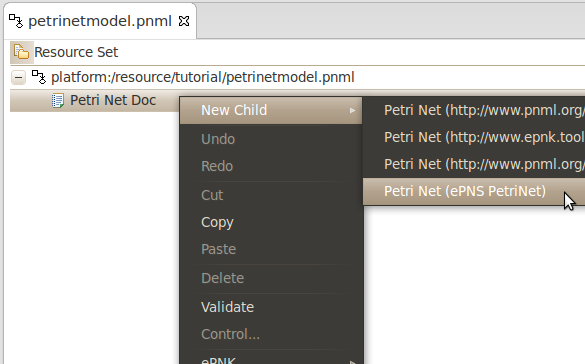
\includegraphics[width=10.0cm]{image/tutorial/Tutorial_01.png}
  \caption{Creation of the Petri net model}
  \label{fig:tut01}
\end{center}
\end{figure}

\begin{figure}[htp]
\begin{center}
  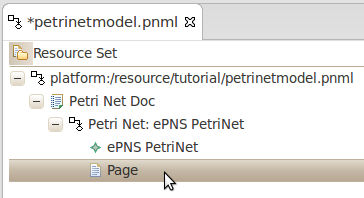
\includegraphics[width=6.0cm]{image/tutorial/Tutorial_02.png}
  \caption{PetriNet Page}
  \label{fig:tut02}
\end{center}
\end{figure}

\begin{figure}[htp]
\begin{center}
  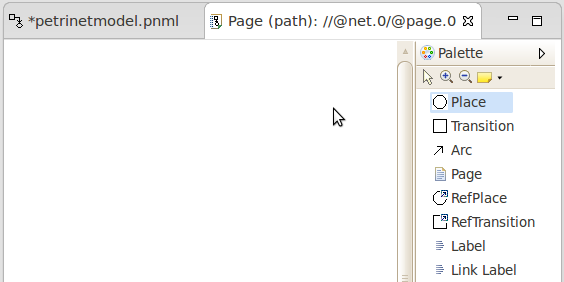
\includegraphics[width=10.0cm]{image/tutorial/Tutorial_03.png}
  \caption{Palette}
  \label{fig:tut03}
\end{center}
\end{figure}

\begin{figure}[htp]
\begin{center}
  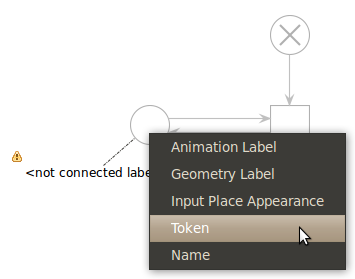
\includegraphics[width=8.0cm]{image/tutorial/Tutorial_04.png}
  \caption{Creation of tokens}
  \label{fig:tut04}
\end{center}
\end{figure}

\newpage 
You should now have a Petri net model similar to the one in Figure \ref{fig:tut05}.

\begin{figure}[htp]
\begin{center}
  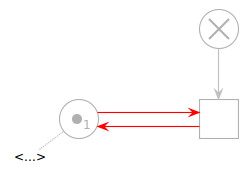
\includegraphics[width=5.0cm]{image/tutorial/Tutorial_05.png}
  \caption{PetriNet model}
  \label{fig:tut05}
\end{center}
\end{figure}

You can now proceed to the Geometry editor \index{editors!geometry}, where you will draw the 2D path along which the 
Token representations (the cube in this example) will move. The Geometry for this particular example will consist of a 
circular line and a separate point (where a button that represents the Input Place will appear in the final visualization
to allow the user to create a new Token in the Input Place to make the Transition fire). 

The following steps describe how to do this:
\begin{enumerate}
  \item Select the project you created before in the Project Explorer and right click on it to select "New > Other > 
  ePNS > Geometry Diagram". Click "Next".
  \item Once again, the project you created should be selected as the parent folder (if it is not, change it). Give 
  your Geometry Diagram a name (keeping the \textit{.geometry\_diagram} extension). Click "Next".
  \item The Geometry Model needs also to be created together with the Geometry Diagram. Select your project as the parent 
  folder and give your Geometry Model a name (keeping the \textit{.geometry} extension). Click "Finish".
  \item The file with the \textit{.geometry\_diagram} extension is the graphical editor. Open it to start building your Geometry.
  \item Create a Track Position on the canvas (in this example, this Track Position will represent the beginning and
  end of the same Track, the only one used, but it could be the beginning of a Track and the end of a different one;
  for more information see \ref{sec:userguide:geometry:elements}), select the Track tool and click on the Track
  Position you just created. A Track with the shape of a square will appear. You can click on the Track and modify
  its shape to create a circle.
  \item Give a name to the Track by filling the Label attached to it, for example "circle".
  \item To create the button that will allow the cube to move, you have to add a SimplePosition (for more information
  on SimplePosition objects, see \ref{sec:userguide:geometry:elements}) to the canvas. Give also a name to this
  element, for example "point".
\end{enumerate}

The Geometry model should now look like Figure \ref{fig:tut06}, where the empty square is the Track Position, the Track
symbol with the word "circle" is the Label and the square with the dashed line and the word "point" is the SimplePosition.

\begin{figure}[htp]
\begin{center}
  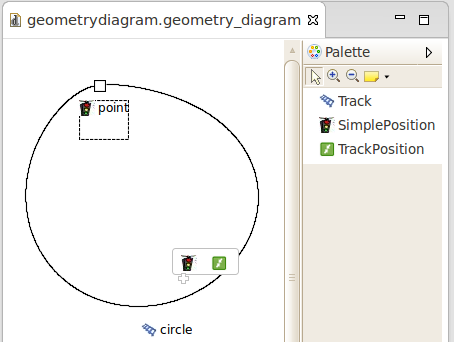
\includegraphics[width=10.0cm]{image/tutorial/Tutorial_06.png}
  \caption{Geometry model}
  \label{fig:tut06}
\end{center}
\end{figure}

Now that you have the Geometry model, you have to specify which Geometry object corresponds to each Place. For this purpose, 
you have to assign a Geometry Label \index{ePNS Petri net!attributes!Geometry Label} to each place of the Petri net model.
\begin{enumerate}
\item Go back to the Petri net graphical editor, create a Label and link it to a Place. You will see that you can set the Label 
to the type "Geometry Label" (See Figure \ref{fig:tut07}), where you must write the name of the correponding Geometry element.
\item Add a \textit{Geometry Label} to the ordinary Place and call it "circle" (See Figure \ref{fig:tut08}).
\item Also add a \textit{Geometry Label} to the Input Place and assign the name "point".
\end{enumerate}

\begin{figure}[htp]
\begin{center}
  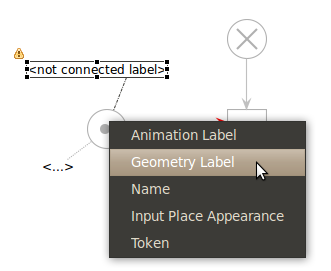
\includegraphics[width=7.0cm]{image/tutorial/Tutorial_07.png}
  \caption{Create Geometry Label}
  \label{fig:tut07}
\end{center}
\end{figure}

\begin{figure}[htp]
\begin{center}
  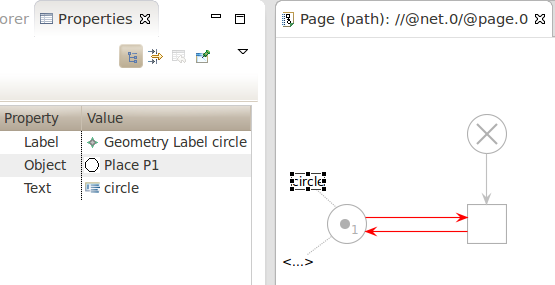
\includegraphics[width=10.0cm]{image/tutorial/Tutorial_08.png}
  \caption{Geometry Label of the ordinary place}
  \label{fig:tut08}
\end{center}
\end{figure}

\newpage
Now, you need to indicate the behaviour of the simulation: when you click on the button, a red cube shall move following the 
circular line at a certain speed. This is done by assigning an Animation \index{animations} to the ordinary Place.
\begin{enumerate} \index{ePNS Petri net!attributes!Animations}
  \item In the Petri net graphical editor, create a Label and connect it to the ordinary Place, selecting "Animation Label"
  (See Figure \ref{fig:tut09}).
  \item As the Label needs a correct Animation, a warning symbol will appear until you write it. To do that, edit the Label 
  and write "move(3.0)" on it. This is to specify that the cube shall move at a speed with the value 3, and it will move along 
  the Track named "circle" because that is the name of the previously created Geometry Label.
\end{enumerate}

\begin{figure}[htp]
\begin{center}
  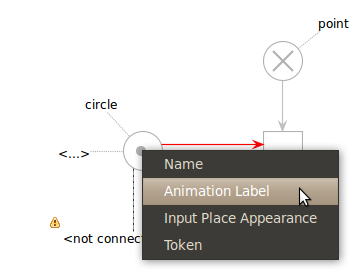
\includegraphics[width=7.0cm]{image/tutorial/Tutorial_09.png}
  \caption{Create Animation Label}
  \label{fig:tut09}
\end{center}
\end{figure}

The Simulator does not know yet how the different elements of the Petri net model should look like. In particular, the Appearance of the
Token (a red cube), the Input Place (a button) and the ordinary Place (a track) should be set. To do this, an Appearance configuration 
has to be created. \index{editors!appearance} \index{appearance}
\begin{enumerate}
  \item Select the project you created before in the Project Explorer and right click on it to select "New > Other > ePNS > 
  Appearance Model". Click "Next".
  \item Once again, the project you created should be selected as the parent folder (if it is not, change it). Give your 
  Appearance Model a name (keeping the \textit{.appearance} extension). Click "Next".
  \item Select "ePNS Appearance Model" as your Model Object and click on "Finish".
  \item Open the file and expand the root node of the tree editor. Right click on "ePNS Appearance Model" and select "New Child > Shape3D". 
  A Shape3D object will appear. \index{appearance!Shape3D}
  \item Open the Properties View of the newly created shape and fill the Label property with a name, for example "cube". In the 
  Type property you will see that you can choose between some different shapes. Select "Cube" (See Figure \ref{fig:tut10}).
  \item To set the color of the shape, right click on its node and select "New Child > Surface Color". In the properties view, modify the Label
  to put a name and select "Red" for the Color attribute (See Figure \ref{fig:tut11}). \index{appearance!Surface Color}
  \item To enhance the way the cube shape will look in the visualization, set the Scale attribute to "10.0" and the Elevation attribute to "9.0".
  \item You also need a shape to model the button. If you have a predefined model, you can use it to represent the button (otherwise you can simply use a Shape3D as done in the previous step). To load an existing model, you need to: \index{appearance!Model3D}
  \begin{enumerate}
    \item Add the model to the Eclipse Workbench by simply dragging and dropping to the project folder (See Figure \ref{fig:tut12}).
    \item Create a new Model3D (right click on "ePNS Appearance Model" and then select "New Child > Model3D") and assign a name to the 
    Label attribute (for example, "button")
    \item Right click on the Model3D and select "Load File...". A resource browser will appear, showing your project folder (See Figure 
    \ref{fig:tut13}). Explore it and select the model for the button you added before (the extensions supported are .obj and .3ds). Click OK.
    \item You may need to change the other attributes of the Model3D (elevation, scale and rotations) later, until it looks nice in 
    the simulation.
  \end{enumerate}
  \item Finally, you need to set the appearance of the track. You can simply choose a color by creating a new Surface Color, or you can also
  select a predefined Texture. To do this: \index{appearance!Texture}
  \begin{enumerate}
    \item Drag and drop the texture file (.jpg and .png extensions supported) to the project folder.
    \item Create a new Texture (right click on "ePNS Appearance Model" and then select "New Child > Texture") and assign a name to the 
    Label attribute (for example, "rail").
    \item Right click on the Texture and select "Load File..." to choose the corresponding texture.
  \end{enumerate}
  \item Now that you have finished the Appearance Model, right click on the root node and select "Validate" (See Figure \ref{fig:tut14}). 
  \index{editors!validation}
  A message saying "Validation Completed Succesfully" should appear.
  \end{enumerate}

\begin{figure}[htp]
\begin{center}
  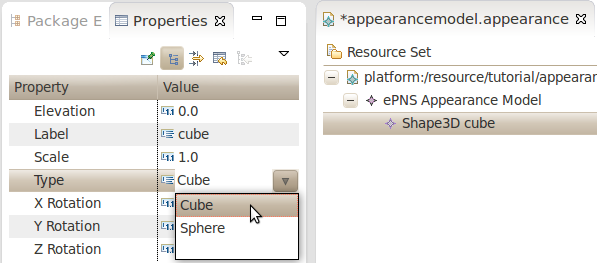
\includegraphics[width=12.0cm]{image/tutorial/Tutorial_10.png}
  \caption{Creation of a cube shape}
  \label{fig:tut10}
\end{center}
\end{figure}

\begin{figure}[htp]
\begin{center}
  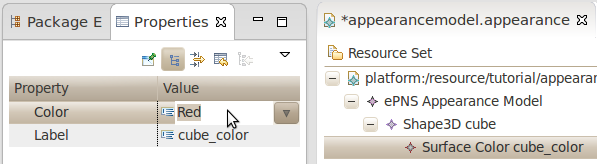
\includegraphics[width=12.0cm]{image/tutorial/Tutorial_11.png}
  \caption{Assigning an color to a shape}
  \label{fig:tut11}
\end{center}
\end{figure}

\begin{figure}[htp]
\begin{center}
  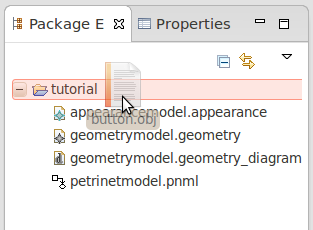
\includegraphics[width=6.0cm]{image/tutorial/Tutorial_12.png}
  \caption{Dragging and dropping a model file to the project folder}
  \label{fig:tut12}
\end{center}
\end{figure}

\begin{figure}[htp]
\begin{center}
  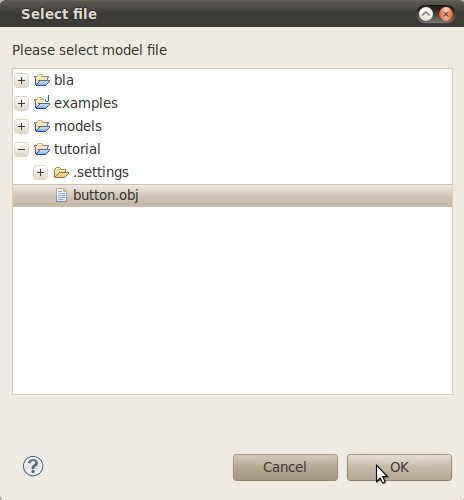
\includegraphics[width=8.0cm]{image/tutorial/Tutorial_13.png}
  \caption{Selecting a model file for the Model3D}
  \label{fig:tut13}
\end{center}
\end{figure}

\begin{figure}[htp]
\begin{center}
  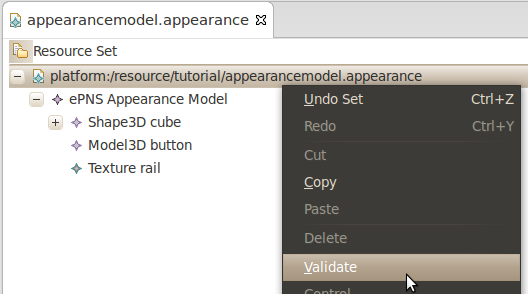
\includegraphics[width=10.0cm]{image/tutorial/Tutorial_14.png}
  \caption{Validating Appearance Model}
  \label{fig:tut14}
\end{center}
\end{figure}

\newpage
Now that all the necessary Appearances are created, you need to connect them to the corresponding elements. The appearance of the Tokens are
specified in the Petri net Model; the remaining Appearances (what Tracks and SimplePositions look like) should be set in the Geometry Model.
\begin{enumerate}
  \item To specify that the Token should look like a cube, you need to go back to the Petri net graphical editor. Edit the Label of the Token you created in the ordinary Place, assigning the name of the previously created shape ("cube") (See Figure \ref{fig:tut15}).
  \item To set the shape of the button, go to the Geometry graphical editor and modify the Appearance attribute of the Simple Position you
  created before (the one with the name "point"). Assign the same name as the corresponding Appearance ("button"). (See Figure \ref{fig:tut16}).
  \item To set the Appearance of the Track, modify the Appearance attribute of the Track "circle" to assign the same name of the
  Appearance ("rail").
\end{enumerate}

\begin{figure}[htp]
\begin{center}
  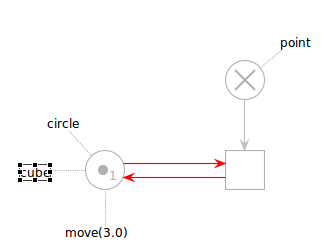
\includegraphics[width=6.0cm]{image/tutorial/Tutorial_15.png}
  \caption{Assigning "cube" appearance to the token}
  \label{fig:tut15}
\end{center}
\end{figure}

\begin{figure}[htp]
\begin{center}
  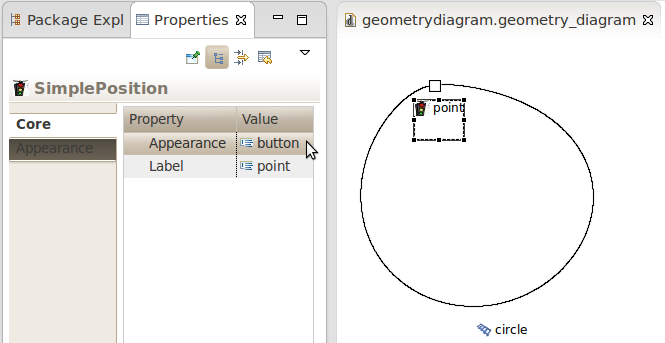
\includegraphics[width=12.0cm]{image/tutorial/Tutorial_16.png}
  \caption{Assigning "button" appearance to the simple position}
  \label{fig:tut16}
\end{center}
\end{figure}

\index{editors!validation}
The models are finished now. You have already checked that the Appearance Model have no errors, but you have to do the same with the 
Geometry and the Petri net Models (right click on the root node of the tree editor and click "Validate"). You will get an error in the 
Petri net Model because the IDs of the Petri net and the Page are not set. Modify them in the Properties View, and validate again. 
This time the validation will success.

Once you have configured the models and the simulation behaviour, you need to connect all the models using the Configurator. \index{configuration}
\begin{enumerate}
  \item Select again the project you created before in the Project Explorer and right click on it to select "New > Other > ePNS > 
  Configurator Model". Click "Next".
  \item Once again, the project you created should be selected as the parent folder (if it is not, change it). Give your Configurator 
  Model a name (keeping the \textit{.configurator} extension). Click "Finish".
  \item Open the file and right click the root node of the tree editor. Select "Load Resource...".
  \item A new window will appear where you can select the files you want to connect (See Figure \ref{fig:tut17}). Click "Browse Workspace...", 
  look for the project you are working in and select the \textit{.pnml} file you created before. Click OK twice to confirm your choice.
  \item Repeat the previous step to add the \textit{.geometry} and \textit{.appearance} files. 
  \item Once you have loaded the three files as resources, you need to attach them to the Configurator. To do this, open the Properties
  View of the Configurator object and edit its three properties selecting the corresponding model (in our case, "ePNS Appearance Model" 
  for ePNS Appearance, "ePNS Geometry" for ePNS Geometry and "Petri Net Doc" for ePNS Petri net) (See Figure \ref{fig:tut18}).
  \item Finally, you can set a default track width for the visualization. Modify the attribute of the Properties View and write "5.0".
\end{enumerate}

\begin{figure}[htp]
\begin{center}
  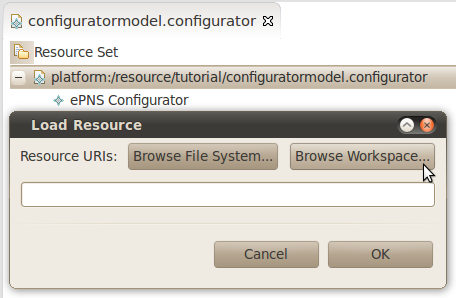
\includegraphics[width=7.0cm]{image/tutorial/Tutorial_17.png}
  \caption{Loading resources}
  \label{fig:tut17}
\end{center}
\end{figure}

\begin{figure}[htp]
\begin{center}
  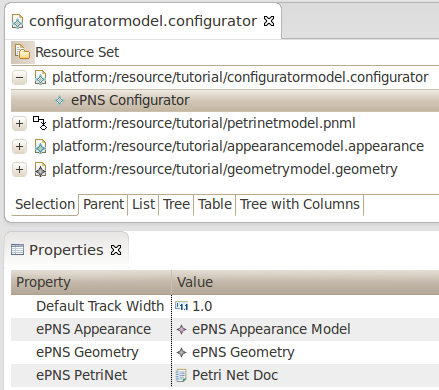
\includegraphics[width=10.0cm]{image/tutorial/Tutorial_18.png}
  \caption{Configurator properties}
  \label{fig:tut18}
\end{center}
\end{figure}

\newpage
By this point, the simulation is ready to be visualized. To start it you must right click on the Configurator object and select 
"Start simulator". \index{simulation}

After starting the Simulator, a new window like the one shown in Figures \ref{fig:tut19} and \ref{fig:tut20} will be displayed. 
Interacting with the simulation can be done in the following steps:
\index{simulation} \index{simulator}
\begin{enumerate}
  \item To start the Graphical Simulation animations, press the Start Button on the left side of the window. 
  \item In order to stop or pause the animation at any point, use the Stop/Pause/Resume\footnote{Please note that Resume is only available 
  after Pause has been clicked, and Stop is only available after Start has been clicked.} buttons available on the top of the window.
  \item Adding a new token in the place set us Interactive Input can be done by just clicking on its representation.
\end{enumerate}

\begin{figure}[htp]
\begin{center}
  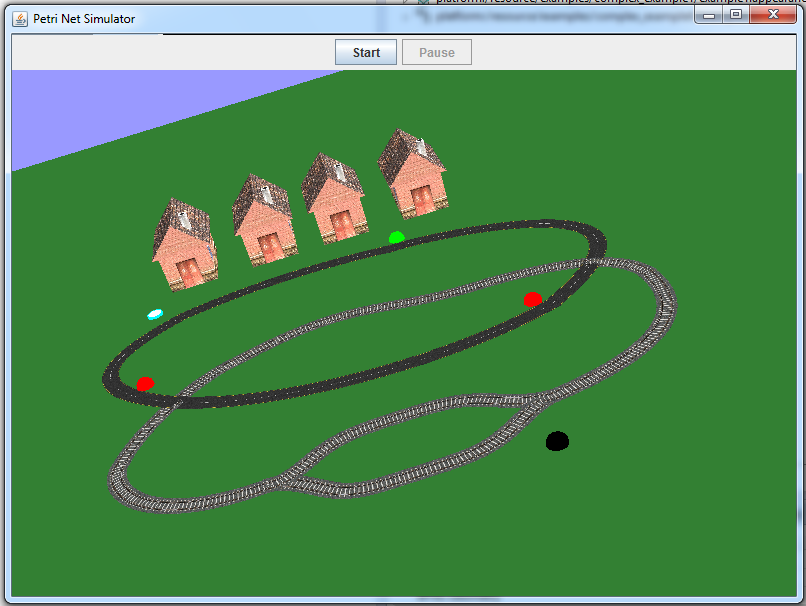
\includegraphics[width=10.0cm]{image/tutorial/Tutorial_19.png}
  \caption{Simulator interface - Before starting}
  \label{fig:tut19}
\end{center}
\end{figure}

\begin{figure}[htp]
\begin{center}
  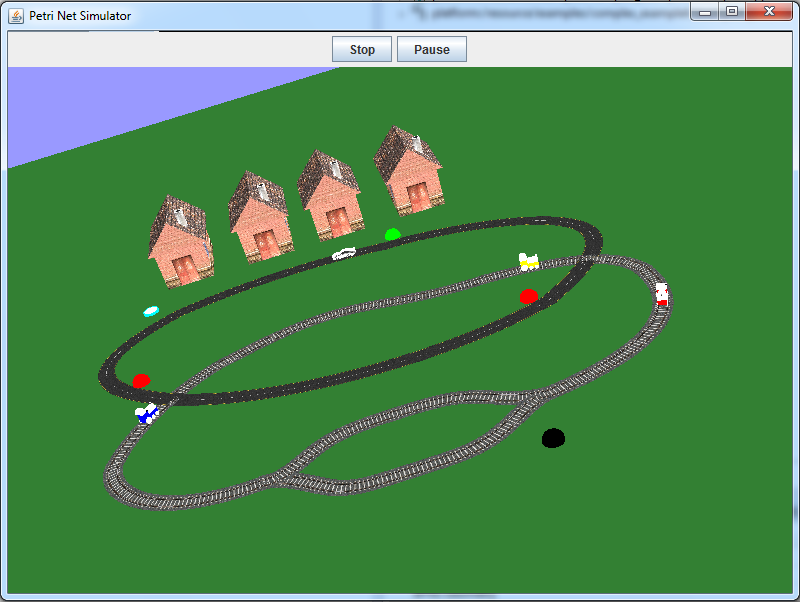
\includegraphics[width=10.0cm]{image/tutorial/Tutorial_20.png}
  \caption{Simulator interface - Simulation running}
  \label{fig:tut20}
\end{center}
\end{figure}

